% Requires graphicx, booktabs, references.bib; paths assume this directory.
% Author-maintained section: the figure renderer does not overwrite this file.
\section{Experimental Validation and Analysis}
\label{sec:eval}

We evaluate QuCl from three perspectives. First, we verify whether the
coupled execution preserves quantum-state continuity, causal event
ordering, and shared-processor timing across ns-3 and NetSquid. Second,
we examine how overlapping quantum operations and classical packet
contention affect the latency and output-state fidelity of a complete
swapping-assisted teleportation workflow. Finally, we quantify the
error introduced when individual execution-coupling mechanisms are
simplified.

One end-to-end workflow consists of entanglement swapping at repeater R,
followed by teleportation from A to B using the same A--B entangled pair.
Q2NS executes the classical protocol and packet delivery in ns-3,
while NetSquid maintains the quantum states and executes the quantum
operations.

\subsection{Experimental Setup}
\label{subsec:eval-setup}

Each experiment executes four end-to-end workflows. Using multiple
workflows creates overlapping demand for the same quantum processors,
while their control packets may simultaneously experience
queueing in the classical network.

We vary two main conditions. The first is the time between workflow
starts, relative to the fixed BSM execution time of 27.405~$\mu$s.
We refer to the three settings as the $0.5\times$, $1\times$, and
$2\times$ intervals: 13.703, 27.405, and 54.810~$\mu$s, respectively.
These factors change the spacing between starts; every workflow still
executes the complete BSM. At $0.5\times$, the next request reaches R
while the preceding BSM is running. At $1\times$ and $2\times$, the
spacing equals or exceeds the BSM duration. The $0.5\times$ interval is
rounded up by 0.5~ns to an integer number of nanoseconds.

The second condition is classical-network contention. Background traffic
is introduced on the R--B link at offered loads of 0, 0.25, 0.50, and
0.75. The zero-load case provides the baseline without background
traffic, while increasing load creates progressively greater opportunity
for the protocol packets to experience queueing. For each nonzero load,
we repeat the experiment with 16 different background-traffic starting
offsets so that the result does not depend on one particular alignment
between background and protocol packets. Background packets carry
1000-byte payloads (1030 bytes on the wire); their period is the
82.4-$\mu$s serialization time divided by the offered load, rounded
to nanoseconds. Protocol traffic is additional to this background load.

The remaining network and quantum parameters are fixed across these
comparisons. The R--A and R--B quantum-delivery times are 0.8 and
1.2~ms, respectively, providing an asymmetric but reproducible resource
delivery condition. Classical links operate at 100~Mb/s with
100~$\mu$s propagation delay. Input qubits and elementary EPR pairs are
created at $t=0$, and the first workflow begins at 2~ms, after the
elementary resources have been delivered. These values are controlled
simulation parameters, kept unchanged while workflow overlap and
classical load are varied.

Table~\ref{tab:qucl-physical-profile} gives the quantum parameters and
their sources. Gate and measurement times follow the simulation profiles
of Liao et al.~\cite{liao2022benchmarking} and Iqbal et
al.~\cite{iqbal2023cloning}. We retain $T_1=20$~ms and $T_2=10$~ms,
values also used by Bugalho et al.~\cite{bugalho2023resource}.
Applying this memory profile uniformly to all positions combines these
sources into an abstract model, rather than reproducing one device.

\begin{table}[t]
\centering
\caption{Quantum parameters and provenance. BSM and correction durations
are derived from the implemented circuit.}
\label{tab:qucl-physical-profile}
\small
\begin{tabular}{@{}lll@{}}
\toprule
Parameter & Value & Source \\
\midrule
CNOT & 20~$\mu$s & \cite{liao2022benchmarking,iqbal2023cloning}, Table~3 \\
H / X / Z & 5~ns & \cite{liao2022benchmarking,iqbal2023cloning}, Table~3 \\
Measurement & 3.7~$\mu$s & \cite{liao2022benchmarking,iqbal2023cloning}, Table~3 \\
Memory $T_1$, $T_2$ & 20, 10~ms & \cite{bugalho2023resource}, Fig.~3a \\
Gate depolarization $p$ & 0.01 & \cite{iqbal2023cloning}, Sec.~4 \\
\midrule
Serial CNOT--H--M--M & 27.405~$\mu$s & QuCl circuit \\
Two correction slots & 10~ns & QuCl circuit \\
\bottomrule
\end{tabular}
\end{table}

NetSquid applies native T1/T2 noise throughout idle and active memory
storage. Independent depolarization,
$\mathcal D_p(\rho)=(1-p)\rho+pI/2$, acts on each gate operand after
that gate's storage interval and immediately before the CNOT, H, X or Z.
Each correction occupies two 5-ns X-or-I and Z-or-I slots, so its duration
is independent of the measurement outcome. Measurements and identity
slots receive storage noise only. Initial states and readout are ideal;
quantum transit is lossless and noiseless. Storage noise begins on memory
placement: at $t=0$ for the input and after transit for delivered halves.

Quantum-state evaluation uses the six Pauli eigenstates
$|0\rangle$, $|1\rangle$, $|+\rangle$, $|-\rangle$, $|+i\rangle$,
and $|-i\rangle$. Swapping and teleportation each produce one of four
possible BSM outcomes, giving 16 possible joint outcome combinations.
The full four-workflow experiment is rerun separately for each input;
we verify that instruction and packet timings are input-independent.
For each input state, a separate NetSquid-only reference evaluates all
16 combinations using the operation times observed in QuCl. Both paths
use NetSquid's native \texttt{fidelity(..., squared=True)} routine to
compute $F=\langle\psi|\rho_B|\psi\rangle$ against the originally
prepared input, including input-memory aging. The reference fidelities
are weighted by the corresponding measurement probabilities, and the
six input states are then averaged equally. Fixed instruction durations
and packet sizes make the execution schedule independent of the sampled
outcomes, allowing all branches to be evaluated at those same times.
This prevents the reported fidelity from depending on a particular
sampled BSM outcome or input state.

For each loaded condition, the four workflows and six input states are
first averaged for each background-traffic offset. We then report the
mean across the 16 offsets together with a 95\% percentile bootstrap
interval from 10,000 resamples. Inputs and workflows are averaged within
an offset, rather than counted as independent traffic samples.
The zero-load condition is deterministic because no background-traffic
alignment is present.

\subsection{Execution Correctness}
\label{subsec:eval-correctness}

\begin{table}[t]
\centering
\caption{Execution validation under the evaluated quantum and network model.}
\label{tab:qucl-validation}
\small
\begin{tabular}{@{}lr@{}}
\toprule
Check & Result \\
\midrule
Input states $\times$ joint outcomes & 6 $\times$ 16 \\
Noiseless chains & 324 \\
Noisy validation runs & 12 \\
Same-qubit handoff / native ownership & PASS \\
Input-independent timing / no drops & PASS \\
Regression and evaluation tests & 240 \\
Max. density-matrix error & $9.99\times 10^{-16}$ \\
\bottomrule
\end{tabular}
\end{table}

Table~\ref{tab:qucl-validation} summarizes the execution checks.
We first verify that QuCl preserves the intended execution across the
two simulators. In the noiseless case, all six input states and all
16 joint BSM outcomes produce the expected teleported state to numerical
precision. With memory and operation noise enabled, intermediate and
final density matrices are compared against the separate NetSquid-only
reference at the same observed operation times.

The validation also checks the execution properties introduced in
Sec.~\ref{sec:design}. The A--B pair produced by swapping must be the
same physical pair later consumed by teleportation, with no duplicate
quantum state maintained on the Q2NS side. Teleportation cannot begin
before the B--R--A readiness packet reaches A, and each correction must
wait for the corresponding measurement-result packet. Processor start,
completion, and waiting times are additionally checked against an
independent capacity-one FIFO reference.

\subsection{End-to-End Latency}
\label{subsec:eval-latency}

% Remove this line if the enclosing manuscript already controls numbering.
\setcounter{figure}{2}
\begin{figure*}[t]
\centering
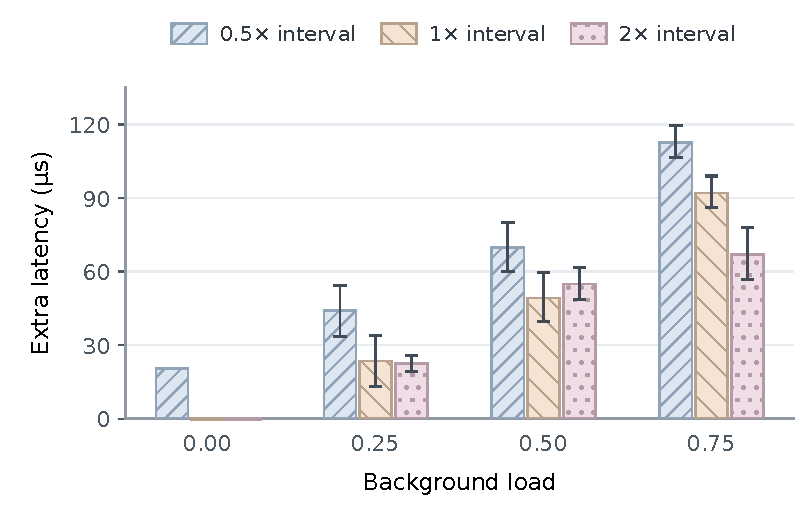
\includegraphics[width=.72\textwidth]{figures/fig3_chain_latency.pdf}
\caption{End-to-end latency of the swapping-assisted teleportation
workflow. The vertical axis shows additional latency relative to the
common unloaded and noncontending reference of 576.110~$\mu$s.
The legend identifies the workflow-start intervals defined in
Sec.~\ref{subsec:eval-setup}.
Error bars show 95\% bootstrap intervals over background-traffic
starting offsets; the zero-load condition is deterministic.}
\label{fig:qucl-chain}
\end{figure*}

Fig.~\ref{fig:qucl-chain} measures the complete execution from the
start of a workflow to the usable teleported output at B. The measured
path includes the swapping BSM at R, delivery of its result to B, the
swapping correction, the B--R--A readiness notification, the teleportation
BSM at A, delivery of its result to B, and the final correction.

Shorter workflow-start intervals increase the overlap among quantum
operations and therefore increase the opportunity for processor
waiting. Increasing the R--B background load independently increases
the opportunity for classical control packets to experience queueing.
Because these two effects occur within the same execution chain,
processor waiting can shift the generation time of a control packet,
which can in turn change the queue state encountered by that packet.

The $0.5\times$ and $1\times$ intervals also illustrate the difference
between request-relative latency and absolute execution time. Although
their requests are generated at different times, serialization through
the capacity-one R processor produces the same absolute completion
schedule in these experiments. Their mean latency differs by
20.553~$\mu$s because the workflow start times differ, rather than because
the quantum state experiences a different absolute execution history.

\subsection{Output-State Fidelity}
\label{subsec:eval-fidelity}

\begin{figure*}[t]
\centering
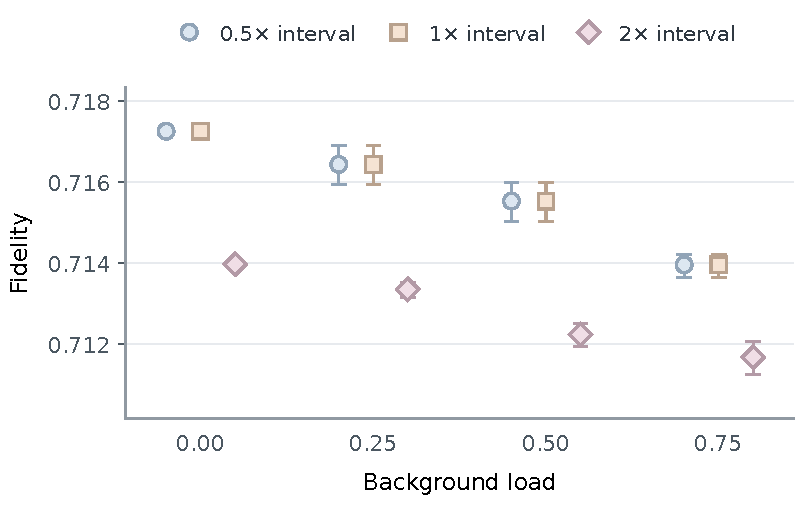
\includegraphics[width=.72\textwidth]{figures/fig4_teleport_fidelity.pdf}
\caption{Final teleportation fidelity, probability-weighted over
16 joint BSM outcomes and equally averaged over six inputs and four
workflows. Whiskers show 95\% phase-bootstrap intervals. The fidelity
axis is expanded to show small differences; all conditions use the same
$T_1=20$~ms, $T_2=10$~ms and gate-noise model.}
\label{fig:qucl-fidelity}
\end{figure*}

Fig.~\ref{fig:qucl-fidelity} evaluates the final teleported state under
the same conditions as Fig.~\ref{fig:qucl-chain}. At the $0.5\times$
interval, the six-input mean fidelity decreases from 0.7172 at zero
background load to 0.7140 at load 0.75. The change results from the
different execution and storage histories produced by the loaded
classical network.

The comparison across workflow-start intervals further shows that
request-relative latency alone does not determine quantum-state quality.
The $0.5\times$ and $1\times$ conditions have equal fidelity within numerical
precision because their quantum resources experience the same absolute
execution times, even though their request-relative latencies differ.
Conversely, at zero background load, the $1\times$ and $2\times$ intervals
have the same mean latency of 576.110~$\mu$s, while their mean
fidelities are 0.7172 and 0.7140, respectively. Their resources were
created at the same initial time but consumed at different absolute
times, producing different memory-aging histories.

This distinction is important because changing the workflow-start
interval changes both execution overlap and the age of resources that
were created at $t=0$. We therefore use comparisons across classical
loads at a fixed start interval when examining the effect of packet
contention, rather than interpreting differences across intervals as
processor contention alone.

\subsection{Simplification Error}
\label{subsec:eval-simplification}

\begin{figure*}[t]
\centering
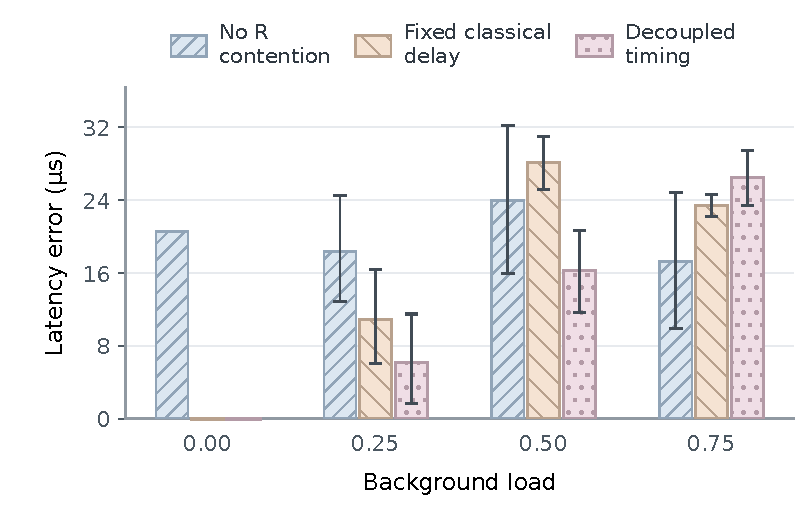
\includegraphics[width=.72\textwidth]{figures/fig5_model_error.pdf}
\caption{Latency error introduced by simplifying execution coupling.
The figure reports swapping-stage mean absolute error (MAE) relative to
Full Sync at the $0.5\times$ workflow-start interval (13.703~$\mu$s).
Error bars show 95\% bootstrap intervals over traffic starting offsets.}
\label{fig:qucl-models}
\end{figure*}

We next isolate the effect of simplifying individual coupling mechanisms
using the swapping stage. Full Sync preserves native packet execution,
quantum-resource timing, and shared-processor execution and serves as
the reference.

No R Contention removes the capacity constraint at the repeater
processor, while still regenerating and transmitting packets at the
resulting operation-completion times. Fixed Classical Delay retains
the shared R processor but replaces the actual result-packet path with
a constant delay obtained from separate calibration runs. Decoupled
Timing combines result-path delays from the No R Contention run with
independently computed FIFO waiting, without regenerating packets after
adding that waiting time. All models use identical workflow starts and
background-traffic offsets.

Calibration uses four disjoint traffic offsets per nonzero load and one
zero-load run, with requests separated by 20 BSM durations. All
calibration packets complete while background traffic remains active.
The reported intervals are conditional on this fixed calibration.

At background load 0.75, the latency MAEs of No R Contention, Fixed
Classical Delay, and Decoupled Timing are 17.28, 23.40, and
26.44~$\mu$s, respectively. In particular, Decoupled Timing misses
the change in packet delay caused by shifting the packet-generation
time. This result demonstrates the cross-domain timing dependence that
QuCl is designed to preserve: quantum execution changes when a control
packet enters the classical network, and the resulting packet delay
affects the next quantum action.

The accompanying swapping-stage analysis also reports Bell-state
fidelity bias for No R Contention and Fixed Classical Delay. This quantity
evaluates the swapping resource itself and is therefore kept separate
from the final teleportation fidelity in Fig.~\ref{fig:qucl-fidelity}.
Decoupled Timing predicts latency only and has no associated
quantum-state estimate.

\paragraph{Scope.}
The evaluation uses a fixed three-node topology, four-workflow batches,
uniform quantum-memory parameters, and controlled periodic background
traffic. The experiments characterize execution correctness and
coupling effects within these conditions. The 5-ms deadline and
$F_{\min}=0.5$ are retained as consistency checks, while the primary
results are the measured latency, output fidelity, and simplification
error described above.
